\section{Straight-line program}
\label{slpsec}
In ambito bioinformatico, una delle principali problematiche è la
gestione di testi molto estesi. Si pensi, ad esempio, al caso umano, dove il
primo cromosoma, il più lungo, conta circa $247.249.719$
\textit{pb} (paia di basi), nonostante l'uomo
non sia l'essere vivente con il genoma più esteso. Fatta questa breve
premessa, è facile comprendere l'importanza degli algoritmi e delle strutture
dati per la compressione di testi.\\
Per questa tesi si è pensato all'uso dei cosiddetti \textbf{straight-line
  program} ($\SLP$). In termini 
generici, un $\SLP$ è una \textit{grammatica context-free} che 
genera una e una sola parola \cite{slpsurvey}. Si parla, quindi, di
\textit{grammar-based compression}.
\begin{definizione}
  Sia dato un alfabeto finito $\Sigma$ di simboli terminali. Sia data una
  stringa $s=a_1,a_2,\ldots, a_n\in\Sigma^{*}$, lunga $n$ e costruita
  sull'alfabeto $\Sigma$, avendo $a_i\in\Sigma$, $\forall\, i \mbox{
    t.c. }1\leq i\leq n$. Si denota con $alph(s)=\{a_1,a_2,\ldots
  a_n\}$ l'insieme dei simboli della stringa $s$.\\
  Si definisce $\SLP$, costruito sull'alfabeto $\Sigma$, una grammatica
  context-free $\mathcal{A}$ tale che: 
  \begin{equation}
    \label{eq:slpdef}
    \mathcal{A}=\left(\mathcal{V}, \Sigma, \mathcal{S}, \mathcal{P}\right)
  \end{equation}
  Dove:
  \begin{itemize}
    \item $\mathcal{V}$ è l'insieme dei simboli non terminali
    \item $\Sigma$ è l'insieme dei simboli terminali
    \item $\mathcal{S}\in \mathcal{V}$ è il simbolo iniziale non terminale
    \item $\mathcal{P}$ è l'insieme delle produzioni, avendo che:
    \begin{equation}
      \label{eq:slpprod}
      \mathcal{P}\subseteq \mathcal{V}\times\left(\mathcal{V}\cup
        \Sigma\right)^{*}
    \end{equation}
  \end{itemize}
  Tale grammatica, per essere un $\SLP$, deve soddisfare due proprietà:
  \begin{enumerate}
    \item si ha una e una sola produzione $(A,\alpha)\in \mathcal{P}$,
    $\forall\, A\in \mathcal{V}$ e con $\alpha\in
    \left(\mathcal{V}\cup\Sigma\right)^{*}$ (si 
    noti che la produzione $(A,\alpha)$ può anche essere indicata con
    $A\to\alpha$) 
    \item la relazione $\{(A,B)\,|\,\,(A,\alpha)\in\mathcal{P},\,\,B\in
    alph(\alpha)\}$ è aciclica
    %\dc{verificare questo secondo punto}
  \end{enumerate}
  Si ha che la grandezza dell'$\,\SLP$ è calcolabile come:
  \begin{equation}
    \label{eq:slplen}
    |\mathcal{A}| = \sum_{(A,\alpha)\in\mathcal{P}}|\alpha|
  \end{equation}
  Il linguaggio $\mathcal{A}$ generato da un $\SLP$ consiste in una singola
  parola, denotata da $eval(\mathcal{A})$. 
\end{definizione}
A partire dall'$\,\SLP$ $\mathcal{A}$ si genera un \textit{albero
  di derivazione}, che, nel dettaglio, è un albero radicato e ordinato
dove la radice è etichettata con $\mathcal{S}$, ogni nodo
interno con un simbolo di $\mathcal{V}\cup\Sigma$ e ogni foglia
con un simbolo di $\Sigma$.
\begin{esempio}
  \label{ese:slpgagie}
  Si prenda, ad esempio \cite{slpgagie}, la seguente stringa:
  \[s=\mbox{GATTAGATACAT}\,\$\mbox{GATTACATAGAT}\]
  Si potrebbe produrre il seguente $\SLP$:
  \begin{multicols}{3}
    \begin{itemize}
      \item $\mbox{S}\to \mbox{ZWAY}\,\$\mbox{ZYAW}$
      \item $\mbox{Z}\to \mbox{WX}$
      \item $\mbox{Y}\to \mbox{CV}$
      \item $\mbox{X}\to \mbox{TA}$
      \item $\mbox{W}\to \mbox{GV}$
      \item $\mbox{V}\to \mbox{AT}$
    \end{itemize}
  \end{multicols}
  Al quale corrisponde il seguente albero di derivazione:
  \begin{figure}[H]
    \centering
    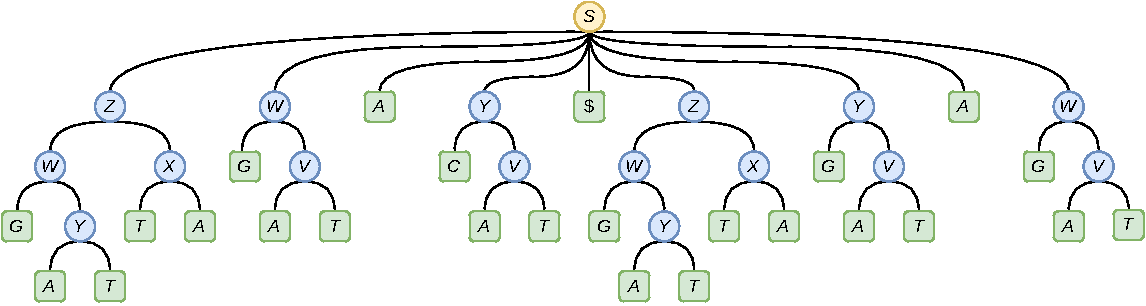
\includegraphics[width=\textwidth]{img/slpgagie.pdf}
  \end{figure}
  Si noti che il simbolo
  iniziale non terminante, ovvero la radice, è indicato con un cerchio giallo, i
  simboli non terminanti, ovvero i nodi interni, sono indicati dai cerchi blu
  mentre i simboli terminanti, ovvero le foglie, sono indicati dai quadrati
  verdi.
\end{esempio}
Nel 2020, Gagie et al. \cite{slpgagie} 
proposero un articolo, a cui si rimanda per approfondimenti, in merito a
miglioramenti prestazionali per il random access all'$\,\SLP$,
anche tramite l'uso dei bitvector sparsi.\\
Si stima che il tempo necessario al random access su un testo $T$, compresso
tramite $\SLP$ e lungo $n$, sia: 
\begin{equation}
  \label{eq:slptime}
  \mathcal{O}\left(\log n\right)
\end{equation}
L'uso degli \textit{SLP} è stato cruciale, come si vedrà più
avanti in questa tesi, per la costruzione della variante run-length encoded sia
della $\BWT$ che della $\PBWT$.
\subsection{Longest common extension}
Oltre a permettere il \textit{random access} al testo compresso, 
l'uso degli $\SLP$ permette di effettuare 
un'altra operazione in modo efficiente, ovvero il calcolo delle \textbf{longest
  common extension} ($\LCE$) \textbf{query}.
\begin{definizione}
  Dato un testo $T$, tale che $|T|=n$, il risultato della $\LCE$ query tra
  due posizioni $i$ e $j$, tali che $0\leq i,j<n$, corrisponde al più lungo
  prefisso comune tra le sottostringhe che hanno come indice di partenza $i$ e
  $j$, ovvero il più lungo prefisso comune tra $T[i,n-1]$ e $T[j,n-1]$.
\end{definizione}
Sfruttando l'$\,\SLP$ del testo $T$ è quindi possibile effettuare due
random access agli indici $i$ e $j$ del testo compresso, per poi ``risalire''
l'albero di derivazione al fine di computare il prefisso comune tra le due
sottostringhe.\\ 
Avendo l'$\,\SLP$ di un testo $T$ lungo $n$, si stima che il calcolo di una
$\LCE$ query di lunghezza $l$ sia
effettuabile in tempo: 
\begin{equation}
  \label{eq:lcetime}
  \mathcal{O}\left(\log n+l\right)\approx\mathcal{O}\left(\log n\right)
\end{equation}
Si noti che, normalmente, la lunghezza dell'$\,\LCE$ è trascurabile rispetto
alla lunghezza 
del testo.\\ 
In questa tesi, i due concetti di $\SLP$ ed $\LCE$ query verranno generalizzati
all'uso su matrici, permettendo una rappresentazione compatta in 
memoria per un pannello di aplotipi, garantendo random access.
\subsubsection{Librerie}
Da un punto di vista implementativo, l'oggetto contenente  l'$\,\SLP$ del
pannello viene costruito e interrogato mediante l'uso della libreria
\textbf{ShapedSlp}\footnote{\url{ttps://github.com/itomomoti/ShapedSlp}},
implementazione dei risultati teorici ottenuti da 
Gagie et al. \cite{slpgagie}. Inoltre, tale libreria basa il suo funzionamento
sull'uso di un'altra libreria, detta
\textbf{BigRePair}\footnote{\url{https://gitlab.com/manzai/bigrepair}}, che 
implementa ulteriori risultati teorici di Gagie et al. \cite{rpair} in merito
alla compressione, via uso di grammatiche, di file con frequenti ripetizioni
(come, nel nostro caso, i pannelli binari di aplotipi).\\
In termini di pipeline, si procede:
\begin{enumerate}
  \item generando la grammatica tramite BigRePair, che accetta
  come file di input un file \texttt{txt} ``raw'' oppure file in formato
  standard nel campo della bioinformatica, come i \texttt{FASTA}
  \item generando l'$\,\SLP$ tramite ShapedSlp specificatamente a
  partire dai risultati di BigRePair (si segnala che la libreria
  accetta anche grammatiche prodotte da altri software).
\end{enumerate}